%%%%%%%%%%%%%%%%%%%%%%%%%%%%%%%%%%%%%%%%%
% Beamer Presentation
% LaTeX Template
% Version 1.0 (10/11/12)
%
% This template has been downloaded from:
% http://www.LaTeXTemplates.com
%
% License:
% CC BY-NC-SA 3.0 (http://creativecommons.org/licenses/by-nc-sa/3.0/)
%
%%%%%%%%%%%%%%%%%%%%%%%%%%%%%%%%%%%%%%%%%

%----------------------------------------------------------------------------------------
%	PACKAGES AND THEMES
%----------------------------------------------------------------------------------------

\documentclass[c]{beamer}
%\documentclass[notes]{beamer}
\setbeamertemplate{note page}[show only notes]
\input{../OR_common.tex}
%%%%%%%%%%%%%%%%%%%%%%%%%%%%%%%%%%%%%%%%%%%%%%%%%%%%%%%%%%%%%%%%%%%%%%%%%%%%%
%%%%%%%%%%%%%%%%%%%%%%%%%%%%%%%%%%%%%%%%%%%%%%%%%%%%%%%%%%%%%%%%%%%%%%%%%%%%%
%%%%%%%%%%%%%%%%%%%%%%%%%%%%%%%%%%%%%%%%%%%%%%%%%%%%%%%%%%%%%%%%%%%%%%%%%%%%%

\title[Introduction]{Unit 1. Introduction to Operational Research. Non linear optimization}

\author{Jordi Villà i Freixa}
\institute[FCTE]{
Universitat de Vic - Universitat Central de Catalunya \\
Study Abroad. Operations Research\\
\medskip
\textit{jordi.villa@uvic.cat}
}
\date{14-28/02, 2023}
\logo{
\includegraphics[width=.1\textwidth]{FCTE}}
\begin{document}

\begin{frame}
\titlepage
\end{frame}


\begin{frame}
    \frametitle{Preliminary}
    This course is strongly based on the monography on Operations Research by Carter, Price and Rabadi \cite{carter}, and in material obtained from different sources (quoted when needed through the slides).
\end{frame}

%%%%%%%%%%%%%%%%%%%%%%%%%%%%%%%%%%%%%%%%%%%%%%%%%%%%%%%%%%%%%%%%%%%%%%%%%%%%%
%%%%%%%%%%%%%%%%%%%%%%%%%%%%%%%%%%%%%%%%%%%%%%%%%%%%%%%%%%%%%%%%%%%%%%%%%%%%%
%%%%%%%%%%%%%%%%%%%%%%%%%%%%%%%%%%%%%%%%%%%%%%%%%%%%%%%%%%%%%%%%%%%%%%%%%%%%%

\begin{frame}
\frametitle{Learning outcomes}
\begin{itemize}
  \item Learn about the origins and applications of Operations Research
  \item Understand system modelling principles
  \item Understand algorithm efficiency and problem complexity
  \item Contrast between the optimality and practicality
  \item Learn about software for operations Research
  \item Introduction to the Python/Colab environment
\end{itemize}
\end{frame}

%%%%%%%%%%%%%%%%%%%%%%%%%%%%%%%%%%%%%%%%%%%%%%%%%%%%%%%%%%%%%%%%%%%%%%%%%%%%%
%%%%%%%%%%%%%%%%%%%%%%%%%%%%%%%%%%%%%%%%%%%%%%%%%%%%%%%%%%%%%%%%%%%%%%%%%%%%%
%%%%%%%%%%%%%%%%%%%%%%%%%%%%%%%%%%%%%%%%%%%%%%%%%%%%%%%%%%%%%%%%%%%%%%%%%%%%%

\section{Nonlinear optimization}

\begin{frame}[t]{Example}{}

  \begin{block}{Production cost}

    A company aims at minimizing the production cost during a series of production periods of time $T_i$, characterised by the demand $D_ii$, equipment capacities and material limitations $E_i$, labor force $L_i$ (which cost depends quadratically on the difference of labor force between two periods $C_L(L_i-L_{i-1})^2$), productivity of each worker $P_i$, the number of units of inventory at the end of each production period $I_i$ and the cost to bring them to the next production period $C_I$.

  \begin{center}
    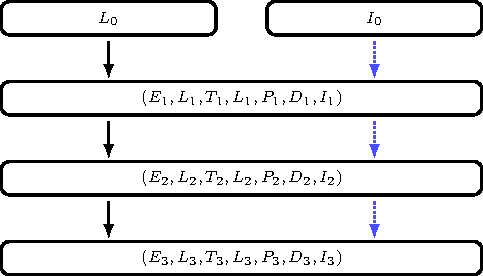
\includegraphics[width=0.4\textwidth]{ProductionSchedule.pdf}
  \end{center}
\end{block}

\end{frame}

\begin{frame}{Example}

  The problem, as stated, aims at minimizing the function:
  \[f(\vec{L},\vec{I})=\sum_{i=1}^T C_L (L_i-L_{i-1})^2+C_I I_i\]
  subject to:
  \[
  \begin{cases}
    L_iP_i \leq E_i\\
    I_{i-1}+L_i P_i \geq D_i\\
    I_i = I_{i-1} + L_i P_i -D_i\\
    L_i,I_i \geq 0, \; \forall i=1,\ldots,T
  \end{cases}
  \]
  Quadratic objective function with linear constraints.

\end{frame}

\begin{frame}{Introduction}

\begin{itemize}
  \item We want to obtain the best solution to a mathematical programming problem in which both  objective function and constraints have general non-linear forms.

  \item Most of the problems are non-linear indeed!

  \begin{itemize}
    \item Unconstrained Problems (often dealt with differential calculus)
    \item Constrained Problems (may include systems of equations to be solved)
  \end{itemize}

  \item Classical underlying mathematical theories do not necessarily provide practical methods suitable for efficient numerical computation.

  \item Points of optimality can be anywhere inside the problem boundaries

  \item No methods applicable to all non-linear problems
\end{itemize}
\end{frame}

\begin{frame}

 \begin{block}{Feasible region}
   Set of points satisfying all the constraints (the area between constraint boundaries).
 \end{block}

 \begin{center}
  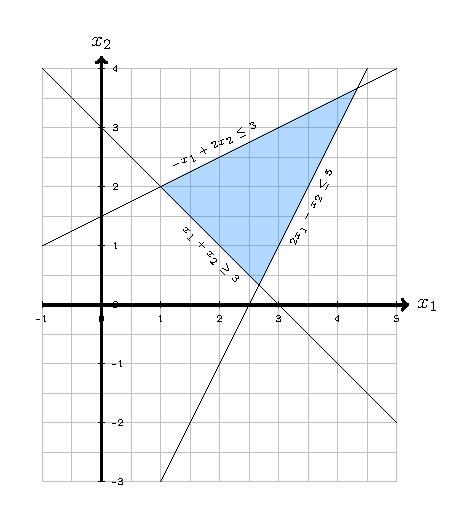
\includegraphics[width=0.6\linewidth]{feasibleregion.pdf}
 \end{center}

\end{frame}
%--- Next Frame ---%

\begin{frame}[t]{Global and local extremes}
  \begin{center}
    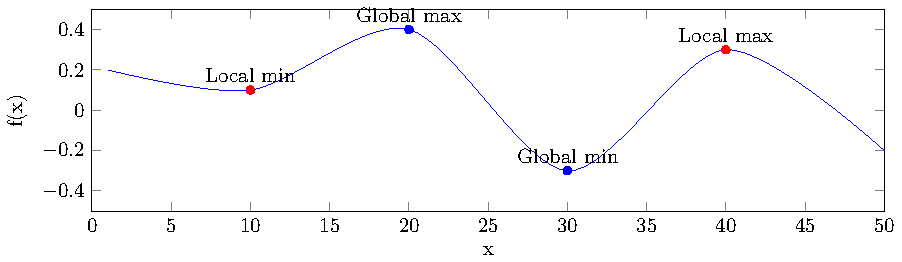
\includegraphics[width=0.6\textwidth]{globalminmax.pdf}
  \end{center}

  A local maximum of the function $f(x)$ exists in $x^*$ if there is a small positive number $\epsilon$ such that
  \[
    f(x^*)>f(x), \; \forall x\in\mathbf{R} : \|x-x^*\| < \epsilon
  \]
  A global maximum of $f(x)$ exists in $x^*$ if
  \[
    f(x^*) > f(x), \; \forall x\in\mathbf{R}
  \]
  (analogous definitions for local/global minimum)
\end{frame}
%--- Next Frame ---%

\subsection{Concavity/convexity}

\begin{frame}[allowframebreaks]
  For a continuous convex function, given any two points $x_1$ and $x_2$:
  \begin{equation}
  f[\lambda x_1 +(1-\lambda)x_2] \leq \lambda f(x_1) +(1-\lambda) f(x_2), \; 0 \leq \lambda \leq 1
\label{eq:convex}
\end{equation}
    (analogous situation for a continuous concave function)
  \begin{center}
    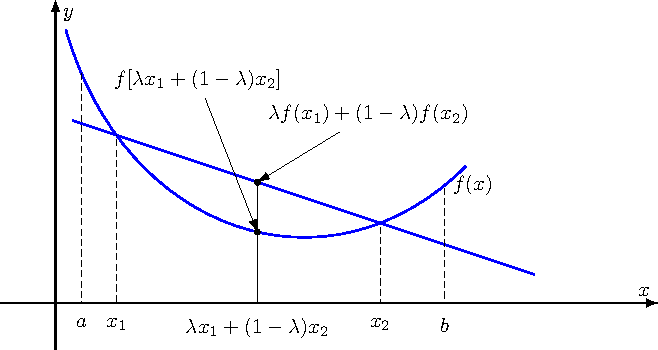
\includegraphics[width=0.6\textwidth]{concave.pdf}
  \end{center}


\begin{block}{Convexity}
    The term "convex" can be applied both to sets and functions. A set $S\in \mathbf{R}^n$ is a {\it convex set} if the straight line segment connecting any two points in $S$ lies entirely inside $S$.
\end{block}
Note that $f(x)$ is a convex function if its domain $S$ is a convex set and if for any two points $x_1$ and $x_2$ in $S$ Eq. \ref{eq:convex} holds.

\begin{Exercise}
  Can you draw a convex function that depends on two variables, $f(x,y)$? Can you generalize Eq. \ref{eq:convex}?
\end{Exercise}

\end{frame}


\begin{frame}[t]
  \begin{itemize}
    \item If a convex nonlinear function is to be optimized without constraints, a global minimum may occur when $f'(x)=0$. Not always this is the case:
    \begin{center}
      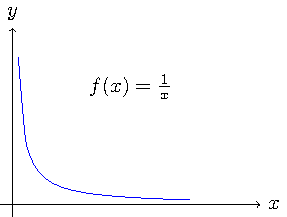
\includegraphics[width=0.5\textwidth]{1overx.pdf}
    \end{center}
    \item If the feasible region for a nonlinear programming problem is convex, each of the constraint functions is convex and are of the form $g_i(x)\leq b_i$
  \end{itemize}

\end{frame}

\begin{frame}[t]{}

  \begin{Exercise}
    Is the function $f(x)=x^2$ convex? Are the regions defined by $x^2=4$ or $x^2\geq 9$ convex?
  \end{Exercise}

\begin{itemize}
    \item A local minimum is guaranteed to be a global minimum for a convex objective function in a convex feasible region, and
    \item a local maximum is guaranteed to be a global maximum for a concave objective function in a convex feasible region.
  \end{itemize}
  Many functions in nonlinear programming problems are neither concave nor convex!
\end{frame}
%--- Next Frame ---%

\begin{frame}[allowframebreaks]{The Hessian matrix}

  \begin{align}
  (\Hessian f)_{ij} &\equiv \frac{\partial^{2} f}{\partial x_{i} \partial x_{j} } \\
  \Hessian\left( \frac{x^{2}}{y} \right) &=
  \begin{bmatrix}
    \frac{2}{y} & - \frac{2x}{y^{2}} \\
    -\frac{2x}{y^{2}} & \frac{2x^{2}}{y^{3}}
  \end{bmatrix}
\end{align}

Let $f$ be a function of $n$ variables and let $1 \leq i \leq n$ and $1 \leq j \leq n$. If the partial derivatives $f'_i$ and $f'_j$ of $f$ exist in an open set $S$ containing $(x_1,\ldots, x_n)$ and both of these partial derivatives are differentiable at $(x_1, \ldots, x_n)$ then $(\Hessian f)_{ij}=(\Hessian f)_{ji}$.

\begin{itemize}
  \item If the Hessian at a given point has all positive eigenvalues, it is said to be a positive-definite matrix. This is the multivariable equivalent of “concave up” (we called it "convex" in this course).
  \item If all of the eigenvalues are negative, it is said to be a negative-definite matrix. This is like “concave down”. (we call it "concave" in this course).
  \item It the eigenvalues are mixed, you have a saddle point.
\end{itemize}
\end{frame}


\begin{frame}
\begin{Exercise}
  Study the critical points of the function $f(x,y)=4x+2y-x^2-3y^2$
\end{Exercise}


\begin{Exercise}
    Check the character of the stationary point in $(0,0)$ for the functions:
    \begin{itemize}
      \item $f(x,y)=x^2+y^2$
      \item $g(x,y)=-x^2-y^2$
      \item $h(x,y)=x^2-y^2$
      \item $k(x,y)=x^3+2y^3-xy$ (is it concave or convex in $(3,3)$? what about in $(-3,-3)$?)
    \end{itemize}

\end{Exercise}

\end{frame}

\begin{frame}{$k(x,y)=x^3+2y^3-xy$}
  \begin{center}
    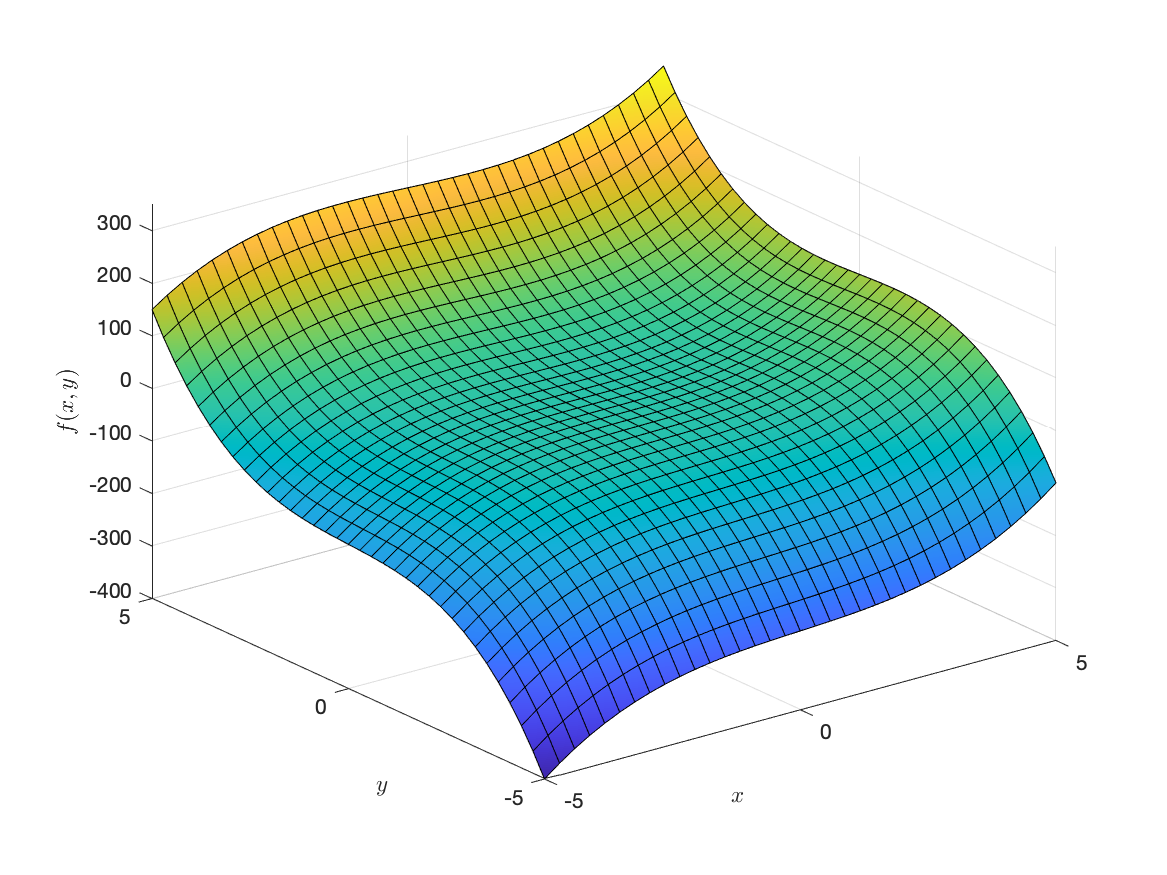
\includegraphics[width=0.8\textwidth]{../figures/x3plus2y3minusxy.png}
  \end{center}
\end{frame}


\begin{frame}{Unconstrained optimization of continuous $f:\mathbf{R}\rightarrow\mathbf{R}$}
  For unconstrained problems with just one variable $x$, if first and second derivatives exist in $x^*$:
  \begin{description}
    \item[Necessary conditions] If $\frac{df}{dx}=0$ at $x=x^*$
    \begin{itemize}
      \item $\frac{d^2f}{dx^2}\geq 0$, for a local minimum at $x=x^*$
      \item $\frac{d^2f}{dx^2}\leq 0$, for a local maximum at $x=x^*$
    \end{itemize}
    \item[Sufficient conditions] If $\frac{df}{dx}=0$ at $x=x^*$
    \begin{itemize}
      \item $\frac{d^2f}{dx^2}> 0$, for a local minimum at $x=x^*$
      \item $\frac{d^2f}{dx^2}< 0$, for a local maximum at $x=x^*$
    \end{itemize}
  \end{description}
\end{frame}
%--- Next Frame ---%

\begin{frame}[allowframebreaks]{Unconstrained optimization of continuous $f:\mathbf{R}^n\rightarrow\mathbf{R}$}
  For unconstrained problems with several variables $\uvec{x}=(x_1,\ldots,x_n)$:
  \begin{description}
    \item[Sufficient condition] If $\pdv{f}{x_i}=0$ at $\uvec{x}=\uvec{x}^*$:
    \begin{itemize}
      \item $\grad{f}=\uvec{0}$, for a local minimum at $x=x^*$ if the function is convex;
      \item $\grad{f}=\uvec{0}$, for a local maximum at $x=x^*$ if the function is concave.
    \end{itemize}
    \item[Decision conditions] The function $f$ is a convex function if $H_f$ is positive definite or positive semidefinite for all $\uvec{x}$; and $f$ is concave if $H_f$ is negative definite or negative semidefinite for all $\uvec{x}$. For $f:\mathbf{R}^2\rightarrow\mathbf{R}$
    \[
      {\mathbf H}_f(x,y)=\begin{pmatrix} \frac{\partial^2 f}{\partial x^2} & \frac{\partial^2 f}{\partial x \partial y} \\ \frac{\partial^2 f}{\partial y \partial x} & \frac{\partial^2 f}{\partial y^2}\end{pmatrix} =
      \begin{pmatrix} A & C \\ C & B \end{pmatrix}
\]
  \end{description}

  Let $f$ be a twice-differentiable function of many variables on the convex open set $S$ and denote the Hessian of $f$ at the point $x$ by $H(x)$. Then
\begin{itemize}
  \item $f$ is concave if and only if $H(x)$ is negative semidefinite $\forall x \in S$
  \item if $H(x)$ is negative definite $\forall x \in S$ then $f$ is strictly concave (see Eq. \ref{eq:convex})
  \item $f$ is convex if and only if $H(x)$ is positive semidefinite $\forall x \in S$
  \item if $H(x)$ is positive definite $\forall x \in S$ then $f$ is strictly convex (see Eq. \ref{eq:convex})
\end{itemize}

\end{frame}

\begin{frame}[t]{Continuity vs derivability}
  Things are not so simple if, for example, functions are not derivable in $x^*$:
  \begin{center}
    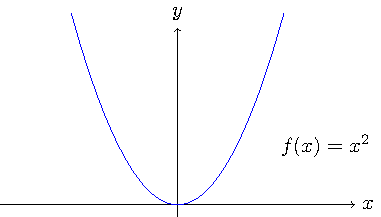
\includegraphics[width=0.4\textwidth]{x2.pdf}
    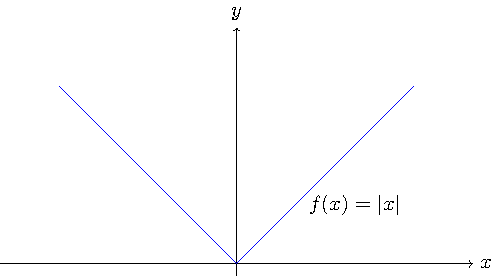
\includegraphics[width=0.4\textwidth]{absx.pdf}
  \end{center}
  Or, if the function is not convex (nor concave), the sufficient condition is lost and we may find local optimal points, instead of global.

  For constrained optimization problems, the shape of the feasible region adds difficulty.
\end{frame}



%--- Next Frame ---%

\subsection{Iterative methods}

\begin{frame}[allowframebreaks]{One-Dimensional line search}
Let us assume a concave function. First, establish error tolerance $\epsilon$. Then:
  \begin{enumerate}
    \item Set up lower and upper bounds for $x$ by finding $x_l,x_u$ such that $\frac{df}{dx_l}\geq 0$ and $\frac{df}{dx_u}\leq 0$
    \item Get new trial intermediate solution (eg, $x=\frac{x_l+x_u}{2}$)
    \item If $x_u-x_l\leq \epsilon$, the terminate
    \item If $\frac{df}{dx}\geq 0$, set $x_l=x$; if $\frac{df}{dx}\leq 0$, set $x_u=x$
    \item Go to step 1
  \end{enumerate}

  For an implementation, see \href{https://machinelearningmastery.com/line-search-optimization-with-python/}{this link}
\end{frame}

\begin{frame}[allowframebreaks]{Golden search method}
For a continuous function it guarantees to find an extremum.

\begin{block}{Golden ratio}
   Two quantities are in the golden ratio if their ratio is the same as the ratio of their sum to the larger of the two quantities:
\[
\frac{a+b}{a}=\frac{a}{b}=\psi \Rightarrow \psi=\frac{1+\sqrt{5}}{2}=1.616033988...
\]
\end{block}

Procedure of the Golden search method, given a function  to be minimized, $f(x)$, the interval to be searched as $x\in(x_1,x_4)$, and their functional values $f(x_1)$ and $f(x_4)$:
\begin{enumerate}
  \item Calculate an interior point and its functional value $f(x_2$). To get the value of $x_2$, ensure the interval lengths are in the ratio $c : r$ or $r : c$ where $r = \phi − 1$; and $c = 1 − r$, with $\phi$ being the golden ratio.
  \item Using the triplet, determine if convergence criteria are fulfilled. If they are, estimate the $x$ at the minimum from that triplet and terminate/return.
  \item From the triplet, calculate the other interior point and its functional value.
  \item The three points for the next iteration will be the one where $f(x)$ is a minimum, and the two points closest to it in $x$.
  \item Go to step 2
\end{enumerate}

\begin{Exercise}
  Use the Golden Search method to find the minimum of function $f(x)=x^2-6x+15$ in the interval $x\in(0,10)$. Set up a spreadsheet to do so.
  %https://www.youtube.com/watch?v=hLm8xfwWYPw
\end{Exercise}

\end{frame}

%--- Next Frame ---%
\begin{frame}[t]{E1. NLO program}
\begin{program}
  E2. Build a Python code that can run one-dimensional search algorithms for user defined functions, using or not first derivatives. Implement the one-dimensional line search and the golden search algorithms and find the optimal solution for the functions:
  \begin{itemize}
    \item $f(x)=x^4-16x^3+45 x^2-20x+203$ within the range $x\in(2.5,14)$
    \item $g(x)=x^5-2x^4-23x^3-12x^2+36x$ within the range $x\in(2,3)$
  \end{itemize}
  Try both a direct implementation as well as the use of solvers in scipy.
\end{program}
\end{frame}



\begin{frame}{Algorithms for unconstrained optimization}
%https://suzyahyah.github.io/calculus/optimization/2018/04/06/Taylor-Series-Newtons-Method.html
  As a reference (not the central aim of this course) here is a list of some algorithms/methods to explore to perform unconstrained optimization in multiple dimensions:
  \begin{itemize}
    \item Newton's method,
    \item Quasi-Newton methods (e.g., \href{https://machinelearningmastery.com/bfgs-optimization-in-python/}{BFGS}),
    \item Trust-region methods,
    \item \href{https://en.wikipedia.org/wiki/Conjugate_gradient_method}{Conjugated gradient methods}.
  \end{itemize}
  and their many variants.
\end{frame}
%--- Next Frame ---%

\subsection{Constrained optimization}

\begin{frame}
In the previous section we have considered functions of several variables that are independent from each other. What happens if the variables are, however, not independent from each other? (see excellent material in \href{https://www.statslab.cam.ac.uk/~rrw1/}{Richard Weber's web site})

  \begin{center}
    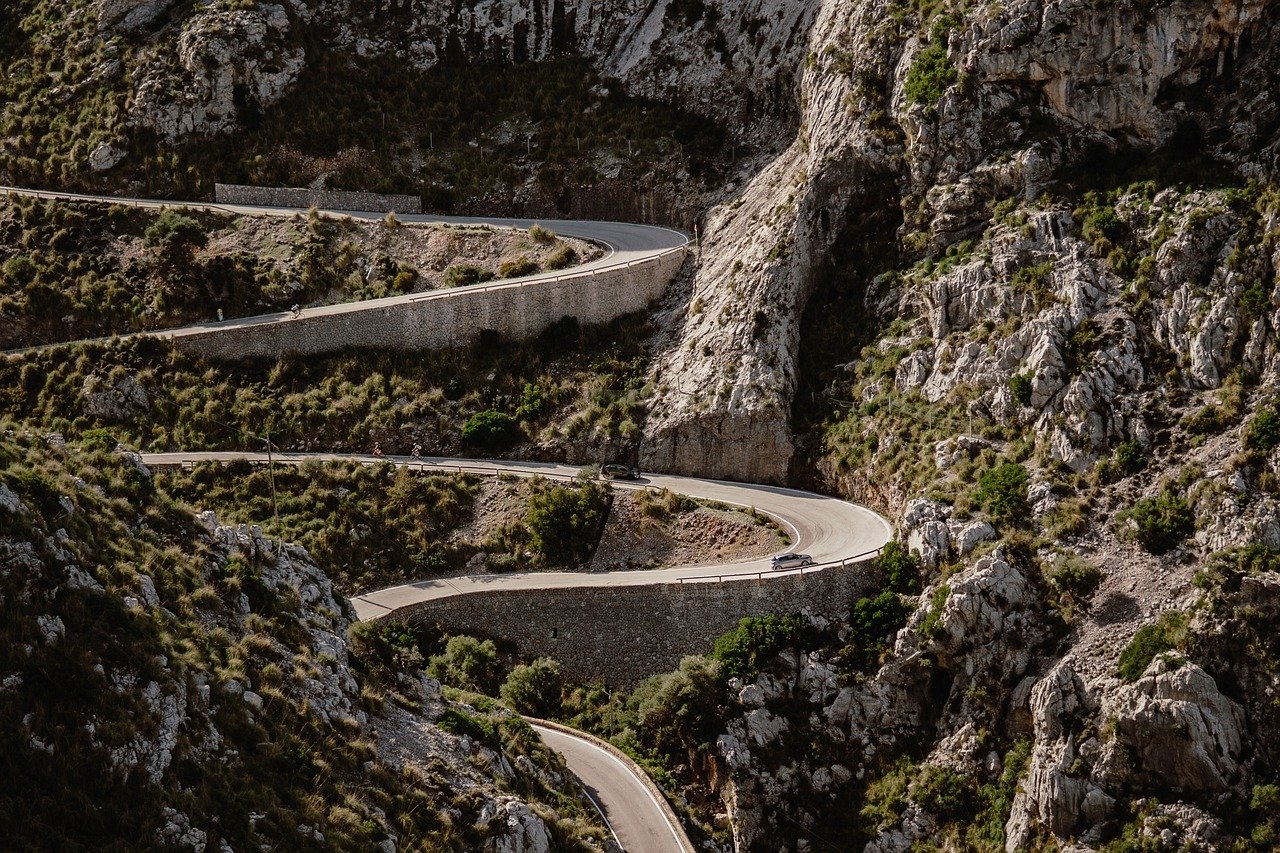
\includegraphics[width=0.7\textwidth]{../figures/mallorca.jpg}\newline
    What is the maximum height we can attain constrained to the trajectory of the road?
  \end{center}
\end{frame}


\begin{frame}[allowframebreaks]{Lagrange multipliers}
  Let us consider optimizing a function $f(x,y)$ (the height of the hill in the previous exemple) subject to the constrain $g(x,y)=c$ (the equation describing the path, the road).

  One can simply substitute $g(x,y)=c$ in $f(x,y)$, but this may not involve trivial algebra.

  Alternatively, let us consider the method of the Lagrange multipliers. To optimize $f(x,y)$ we require
  \[
    df=\frac{\partial f}{\partial x} dx +\frac{\partial f}{\partial y}dy=0
  \]
  we saw that if $dx$ and $dy$ were independent, $\frac{\partial f}{\partial x}=\frac{\partial f}{\partial y}=0$. But they are not here: they are constrained by $g(x,y)$, which is a constant:
  \[
    dg=\frac{\partial g}{\partial x} dx +\frac{\partial g}{\partial y}dy=0
  \]
  Let us consider a parameter $\lambda$ (the {\it Lagrange multiplier}) and obtain an expression for which $dx$ and $dy$ are independent:
  \[
    d(f+\lambda g)=(\frac{\partial f}{\partial x}+\lambda \frac{\partial g}{\partial x}) dx +(\frac{\partial f}{\partial y}+\lambda \frac{\partial g}{\partial y})dy=0
  \]
  Now:
  \begin{eqnarray*}
    \frac{\partial f}{\partial x}+\lambda \frac{\partial g}{\partial x} &=&0\\
    \frac{\partial f}{\partial y}+\lambda \frac{\partial g}{\partial y} &=&0\\
    g(x,y)&=&c
  \end{eqnarray*}
  are sufficient to find $\lambda$, $x^*$ and $y^*$.

\end{frame}

\begin{frame}[allowframebreaks]
  \begin{center}
  \includegraphics<2>[width=0.4\textwidth]{../figures/Lagrangex2minusy.png}
  \end{center}
  \begin{Exercise}
  Find the optimal values of the function $f(x,y)=x^2-y$ constrained within the circumference $x^2+y^2=4$. (note that, interestingly, in the optimal value $x^*$ we will get a gradient for the constraint that is parallel to the gradient of the function: $\grad f(x^*)=\lambda^* \grad g(x^*)$).
\end{Exercise}
\end{frame}

\begin{frame}
  The general problem we study takes the form
  \begin{center}
  \begin{tabular}{cc}
    maximize & $f(x)$ \\
    subject to & $\begin{cases}x\in X\\g(x)=b\end{cases}$
  \end{tabular}
\end{center}
where
  \begin{center}
  \begin{tabular}{rl}
    $x \in \mathbf{R}^n$ & ($n$ decision variables)\\
    $f: \mathbf{R}^n \rightarrow \mathbf{R}$ & (objective function)\\
    $X \subseteq  \mathbf{R}^n$ & (regional constraints) \\
    $\begin{rcases}
      g: \mathbf{R}^n \rightarrow \mathbf{R}^m\\
      b \subseteq \mathbf{R}^m
    \end{rcases}$ & ($m$ functional constraints)\\
  \end{tabular}
\end{center}
If the constraint is $g(x)\leq b$ we introduce a {\bf slack variable} $z$ and write:
\[g(x)+z=b, \, z\geq0\]
Regional and functional constraints define the {\bf feasible set} for $x$

\end{frame}

\begin{frame}[allowframebreaks]{Case when $\uvec{g}(\uvec{x})= 0$: The Lagrangian}

  In the Lagrange approach, the constrained maximization (minimization) problem is rewritten as a Lagrange function 
  
  \[L(x,\lambda)=f(x)-\lambda g(x)\]
  
  whose optimal point is a saddle point, i.e. a global maximum (minimum) over the domain of the choice variables and a global minimum (maximum) over the multipliers.

  Let us take this example:
  \begin{center}
  \begin{tabular}{cc}
    maximize & $f(x)=x_1-x_2-2x_3$ \\
    subject to & $\begin{cases}x_1+x_2+x_3=5\\x_1^2+x_2^2=4\\x=(x_1,x_2,x_3)\in \mathbf{R}^3\end{cases}$
  \end{tabular}
\end{center}
\begin{enumerate}
  \item We write the Lagrangian as (note we have two constraints):
  \begin{eqnarray*}
    L(x,\lambda)&=&x_1-x_2-2x_3-\lambda_1 (x_1+x_2+x_3-5)-\lambda_2(x_1^2+x_2^2-4)\\
    &=& [x_1(1-\lambda_1)-\lambda_2x_1^2]+[x_2(-1-\lambda_1)-\lambda_2x_2^2]+[x_3(-2-\lambda_1)]\\
    &&+5\lambda_1+4\lambda_2
  \end{eqnarray*}
  \item We want to minimize the Lagrangian subject to the regional constraints $x=(x_1,x_2,x_3)\in \mathbf{R}^3$.
  \item We find the values $\lambda$ such that will define a feasible set
  \[
  Y=\left\{\lambda: \underbrace{\mathrm{min}}_{x\in  \mathbf{R}^3} L(x,\lambda) >-\infty \right\}
  \]
  So, we only consider the values of $\lambda$ for which we obtain a finite minimum. In the example
  \[
  Y=\left\{\lambda: \lambda_1=-2, \lambda_2<0 \right\}
  \]
  \item For $\lambda \in Y$, the minimum will be obtained at some $x(\lambda)$ (that depends on $\lambda$ in general). Here, $x(\lambda)=(3/2\lambda_2,1/2\lambda_2,x_3)^T$.
  \item Finally, we find a $\lambda$ value that provides a feasible value $x(\lambda)$. Here
  \[
    x_1^2+x_2^2=4 \Rightarrow \lambda_2 = -\sqrt{5/8}
  \]
  So, $x^*$ is optimal:
  \[
    x^* =(-3\sqrt{2/5},-\sqrt{2/5},5+4\sqrt{2/5})^T; \, \lambda^*=(-2,-\sqrt{5/8})^T
  \]
\end{enumerate}

\end{frame}

\begin{frame}{what if $\uvec{g}(\uvec{x})\geq 0$? Karush-Kuhn-Tucker theorem}
% https://en.wikipedia.org/wiki/Karush%E2%80%93Kuhn%E2%80%93Tucker_conditions
  \note[item]{\url{https://people.maths.bris.ac.uk/~maxmr/opt/kt1.pdf}}
  \note[item]{\url{https://www.cmi.ac.in/~madhavan/courses/dmml2018/literature/Lagrangian_Methods_for_Constrained_Optimization.pdf}}

  Let us consider a general optimization problem with constraints: let $f:\mathbf{R}^n \rightarrow \mathbf{R}$ be the objective function and $\uvec{g}:\mathbf{R}^n \rightarrow \mathbf{R}^m$ a set of constraint functions ($\uvec{g}(\uvec{x})=(g_1(\uvec{x}),\ldots,g_m(\uvec{x}))$ with $\uvec{x}=(x_1,\ldots,x_n)$. We want to obtain
  \begin{center}
  Min $f(\uvec{x})$ such that $\uvec{g}(\uvec{x})\geq 0$
\end{center}
  \begin{theorem}
    If $\uvec{x}^*$ is a local minimum for the optimisation problem and the constraints $\uvec{g}(\uvec{x})\geq 0$ are satisfied at $\uvec{x}^*$, then $\uvec{x}^*$ must satisfy:
    \begin{eqnarray*}
      \grad f({\uvec{x}})&=&\lambda_1 \grad g_1(\uvec{x})+\cdots+\lambda_m \grad g_m(\uvec{x})\\
      0&=&\lambda_1  g_1(\uvec{x})+\cdots+\lambda_m  g_m(\uvec{x})\\
      0&\leq&\uvec{g}(\uvec{x})
    \end{eqnarray*}
  \end{theorem}

\end{frame}


\begin{frame}[allowframebreaks]
    \begin{Exercise}
  Maximize $f(x,y)=xy$ subject to $100 \geq x+y$ and $x\leq 40$.
\end{Exercise}
%https://www.sfu.ca/~wainwrig/Econ400/lecture-notes-Kuhntucker.pdf
\end{frame}
%--- Next Frame ---%
%------------------------------------------------%------------------------------------------------
%------------------------------------------------%------------------------------------------------
%------------------------------------------------%------------------------------------------------
%------------------------------------------------%------------------------------------------------
%------------------------------------------------%------------------------------------------------
%------------------------------------------------%------------------------------------------------
%------------------------------------------------%------------------------------------------------
%------------------------------------------------%------------------------------------------------
%------------------------------------------------%------------------------------------------------
%------------------------------------------------%------------------------------------------------

\section{References}
\begin{frame}{References}
    \footnotesize
    \begin{thebibliography}{99}
    \setbeamertemplate{bibliography item}[text]
      \begin{columns}[t]
        \begin{column}{.45\textwidth}
            \bibitem{carter} Michael W. Carter, Camille C. Price, and Ghaith Rabadi. Operations Research, 2nd Edition. CRC Press.
            \bibitem{harel} David Harel, with Yishai Feldman. Algorithmics: the spirit of computing, 3rd Edition. Addison-Wesley.
            \bibitem{rardin} Ronald L. Rardin. Optimization in Operations Research, 2nd Edition. Pearson.
            \bibitem{hefferon} J. Hefferon. \href{http://joshua.smcvt.edu/linearalgebra}{Linear algebra (4th Ed)}.
        \end{column}
        \begin{column}{.45\textwidth}
            \bibitem{riley} K.F. Riley, M.P. Hobson, S.J. Bence. Mathematical Methods for Physics and Engineering (2nd Ed). McGraw Hill.
            \bibitem{nocedal} J. Nocedal, S. J. Wright. Numerical Optimization (2nd Ed). Springer.
            \bibitem{beers} Kenneth J. Beers. Numerical methods for chemical engineering: applications in Matlab. Cambridge University Press.
            \bibitem{barber} D. Barber. Bayesian reasoning and machine learning. Cambridge University Press.
        \end{column}
      \end{columns}
    \end{thebibliography}
\end{frame}
%----------------------------------------------------------------------------------------

\end{document}
